\chapter{Computando sucesiones aproximativas}
En este capítulo vamos a dise\~nar un programa que nos permita calcular explícitamente sucesiones aproximativas finitas para ciertos espacios. 

Sea $ \mathbb{S}^1  $ la circunferencia unidad. Podemos conseguir una sucesión aproximativa finita tomando $ \eps_n = (2\pi )/n$ y considerando las $ \eps_n  $-aproximaciones $ A_n = \{e^{im \eps_n }\mid m =0,...,n-1\} $. Para definirlas en nuestro programa, simplemente a\~nadimos cada punto a una lista que conforme la aproximación: 
\iffalse
\begin{minted}{python}
    def crearnubecircunferencia(epsilon):
        nube = [];
        theta = 0;
        dospi = 2*math.pi;
        while theta<dospi:
            nube += [[math.cos(theta),math.sin(theta)]];
            theta += epsilon;
        return nube
\end{minted}
\fi 
En vez de calcular primero el espacio finito $ U_{2\eps_n}(A_n) $ y luego representarlo, vamos a dise\~nar un programa que cree el espacio como grafo directamente, y luego lo represente como diagrama de Hasse. 

En vez de trabajar constantemente con los puntos de la aproximación, vamos a trabajar con el conjunto $ \{1,...,n\} $ de números naturales en biyección con la aproximación, y almacenar las distancias entre puntos en una matriz:
\begin{minted}{python}
    def dist(z,w):
    # Calculamos la distancia euclídea entre ambos puntos
    distancia =math.sqrt((z[0]-w[0])**2+(z[1]-w[1])**2);
    return distancia

    def matdist(nube):
        # Creamos una matriz de ceros
        distancias = np.zeros((n,n));
        for i in range(n):
            for j in range(n):
                if i < j:
                    # Introducimos d(z_i,z_j) en la posición (i,j)
                    d = dist(nube[i],nube[j]);
                    distancias[i][j] = d;
                    distancias[j][i] = d;
    return distancias
\end{minted}

Para crear el grafo, recordamos que este tiene por vértices los conjuntos de diámetro menor que $ 2\eps_n  $ y hay una arista $ A\lra B  $ si $ A\subc B  $. La idea de la construcción es la siguiente:
\begin{enumerate}
    \item Empezamos introduciendo los conjuntos unitarios $ \{i\} $.
    \item Para cada par de nodos $ A,B  $ en esta lista, comprobamos si su unión tiene diámetro menor que $ 2\eps_n  $. Si es así, introducimos dicha unión como nodo y registramos $ (A,A\cup B ) $ y $ (B,A\cup B ) $ como lados.
    \item Iteramos el proceso hasta llegar a los nodos de longitud $ n-1 $ (subconjuntos de $ A_n  $ de cardinal $ n-1  $), que ya solo pueden dar $ A_n  $ como nodo.

\end{enumerate}

Esta idea mejora con las siguientes observaciones:
\begin{enumerate}
    \item Si en una iteración no introducimos ningún nodo, hemos de parar, puesto que no habrá conjuntos de mayor cardinal con diámetro menor que $ 2\eps_n  $.
    \item Si $ A\cup B = C  $ y en la siguiente iteración $ A'\cup B' = C  $, con $ A \subc A'  $, podríamos obtener $ (A,C ) $ y $ (A',C ) $ como lados, aunque en el diagrama de Hasse no constaría el primero. Esto se puede evitar introduciendo solamente $ A\cup B  $ cuando su cardinal sea uno por encima del de $ A  $ y $ B  $.
\end{enumerate}

\begin{minted}{python}
    # Calculamos el diámetro con la matriz de distancias
    def diam(C):
        listadistancias = [];
        m = len(C);
        if m == 0 or m == 1:
            return 0
        else:
            for i in range(m):
                for j in range(i+1,m):
                    listadistancias.append(matrizdistancias[C[i]][C[j]])
            return max(listadistancias)
    
    # Construimos el grafo del espacio
    def construirgrafo(nube):
    listanodos = [];
    listalados = [];
    doseps = 2*epsilon;
    n = len(nube);
    # Introducimos los conjuntos unitarios como nodos
    for i in range(n):
        listanodos.append((i,));

    # Recuento de nodos que introducimos en la iteración anterior
    listanodos1 = listanodos; 

    # Iteramos en el número de puntos de la aproximación
    for i in range(n-1):
        l = len(listanodos1);
        # Si en la iteración anterior no introdujimos ninguno, paramos:
        if l == 0:
            break;
        # Almacenamos los que introducimos en esta iteración
        listanodos2 = []; 
        for k in range(l):
            a = listanodos1[k]; # tomamos un conjunto
            for j in range(k+1,l):
                b = listanodos1[j]; # tomamos otro
                aubsinorden = list(set(a).union(set(b))); #unimos
                aub = tuple(sorted(aubsinorden)); #ordenamos cifras

                # Comprobamos que la longitud sea solo una por encima
                if len(aub)>len(a)+1:
                    continue;
                # Comprobamos que no es redundante
                if a == aub or b == aub: 
                    continue;
                # Introducimos el conjunto 
                if diam(aub)<doseps:
                    if aub not in listanodos2:
                        listanodos2.append(aub);
                        listanodos.append(aub);
                    if (a,aub) not in listalados:
                        listalados.append((a,aub));
                    if (b,aub) not in listalados:
                        listalados.append((b,aub));
        # Actualizamos la lista de reserva
        listanodos1  = listanodos2; 
    # Creamos el grafo
    G = nx.DiGraph();
    G.add_nodes_from(listanodos);
    G.add_edges_from(listalados);
    return G
\end{minted}

Por último, reducimos el diagrama de Hasse a su forma minimal, lo cual simplifica la representación y da más información sobre su tipo topológico. Lo hacemos comprobando si hay puntos de subida o bajada según sus predecesores y elimándolos en tal caso, en un proceso recurrente que recorre todos los nodos del grafo.

\begin{minted}{python}
    def hacerminimal(G):
    i=0;
    numnodos = len(list(G.nodes));
    while i<numnodos and numnodos>1:
        nodo = list(G.nodes)[i];
        # Obtenemos su lista de sucesores
        sucesores = list(G.successors(nodo));
        # Obtenemos su lista de predecesores
        predecesores = list(G.predecessors(nodo));

        # Analizamos el caso en el que es un punto colapsable hacia arriba
        if len(sucesores) == 1:
            sucesor = sucesores[0];
            lista1 = [];
            G.remove_node(nodo) # lo eliminamos
            for n in predecesores:
                # añadimos nuevos lados 
                lista1.append((n,sucesor)); 
            G.add_edges_from(lista1);
            return hacerminimal(G) # volvemos a inciar el proceso

        # Analizamos el caso en el que es un punto colapsable hacia abajo
        elif len(predecesores) == 1:
            predecesor = predecesores[0];
            lista1 = [];
            G.remove_node(nodo); # lo eliminamos
            for n in sucesores:
                lista1.append((predecesor,n)); # añadimos nuevos lados 
            G.add_edges_from(lista1);
            return hacerminimal(G) # volvemos a inciar el proceso 
        else:
            i = i+1;
    return G
\end{minted}

Podemos ver un ejemplo ejecutando este código para $ n = 7,..., 15$:
\begin{figure}[h]
    \begin{subfigure}{.5\textwidth}
      \centering
      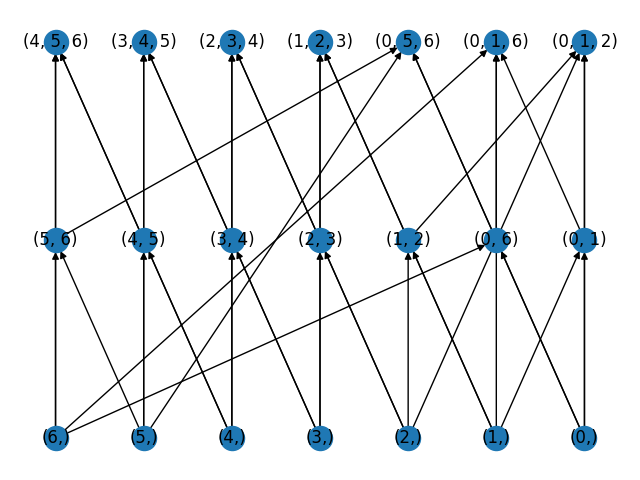
\includegraphics[width=.8\linewidth]{7.png}
      \caption{$n = 7$}
    \end{subfigure}%
    \begin{subfigure}{.5\textwidth}
      \centering
      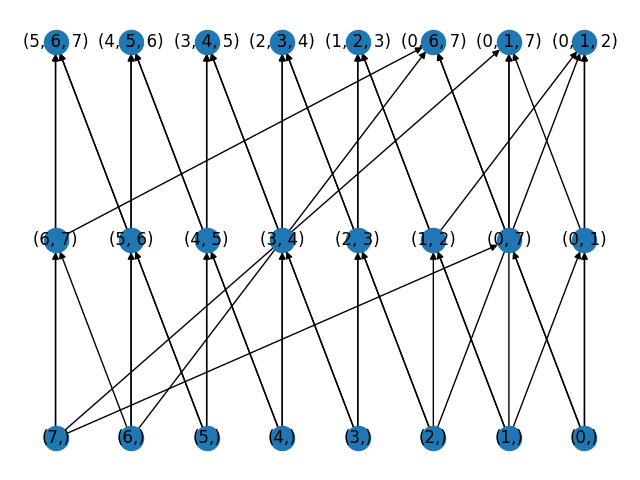
\includegraphics[width=.8\linewidth]{8.png}
      \caption{$ n = 8 $}
    \end{subfigure}
    \begin{subfigure}{.5\textwidth}
        \centering
        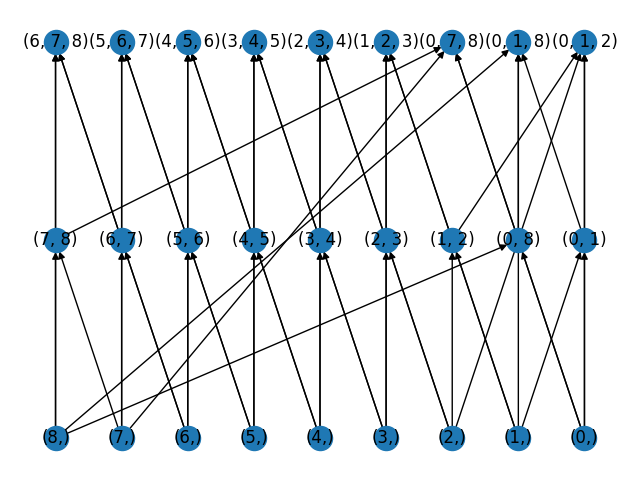
\includegraphics[width=.8\linewidth]{9.png}
        \caption{$ n = 9 $}
      \end{subfigure}%
      \begin{subfigure}{.5\textwidth}
        \centering
        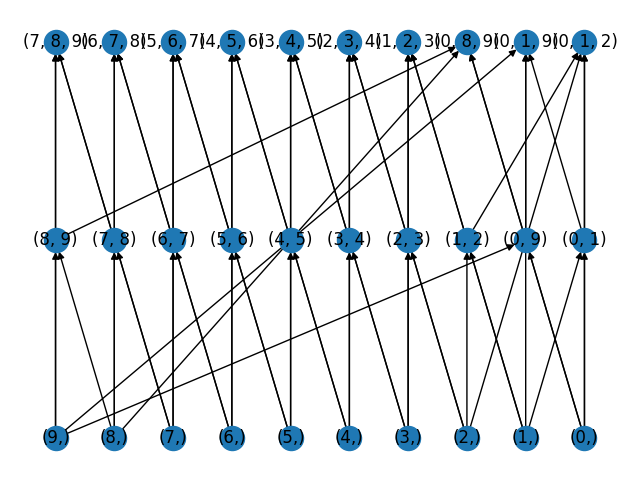
\includegraphics[width=.8\linewidth]{10.png}
        \caption{$ n = 10 $}
      \end{subfigure}
\end{figure}
\begin{figure}[h]
     \begin{subfigure}{.5\textwidth}
        \centering
        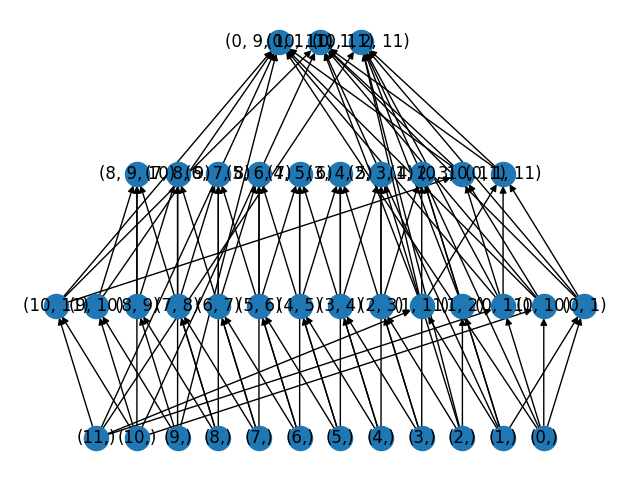
\includegraphics[width=.8\linewidth]{11.png}
        \caption{$ n = 11 $}
      \end{subfigure}%
      \begin{subfigure}{.5\textwidth}
        \centering
        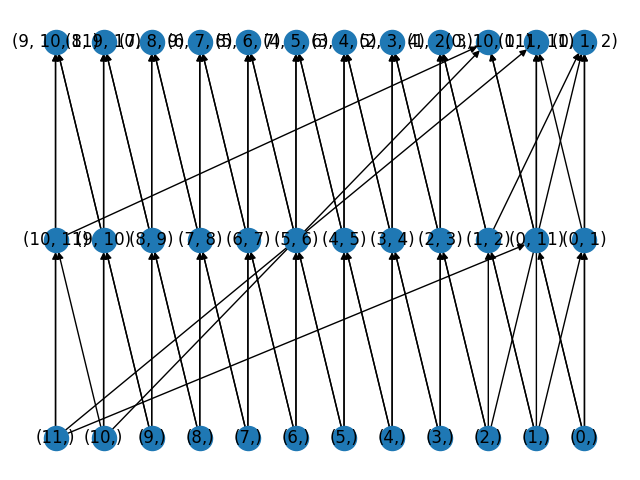
\includegraphics[width=.8\linewidth]{12.png}
        \caption{$ n = 12 $}
      \end{subfigure}
\end{figure}
\begin{figure}[h]
      \begin{subfigure}{.5\textwidth}
        \centering
        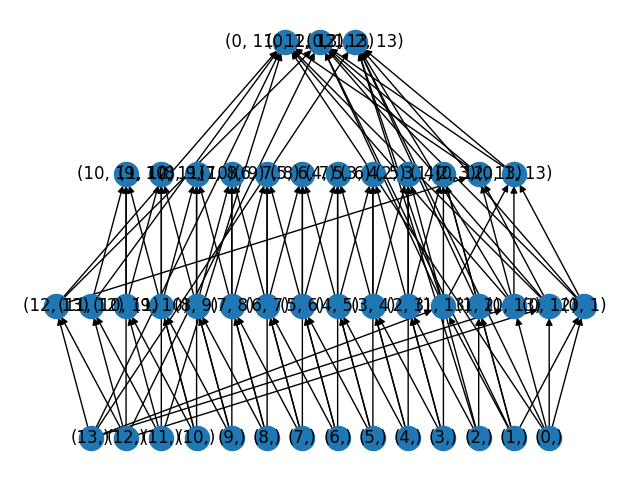
\includegraphics[width=.8\linewidth]{13.png}
        \caption{$ n = 13 $}
      \end{subfigure}%
      \begin{subfigure}{.5\textwidth}
        \centering
        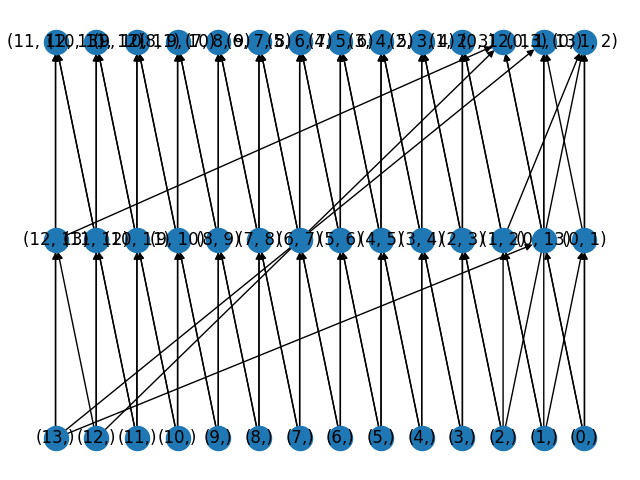
\includegraphics[width=.8\linewidth]{14.png}
        \caption{$ n = 14 $}
      \end{subfigure}
    \caption{Distintas fases de la sucesión aproximativa de la circunferencia.}
    \label{circunferencia}
\end{figure}
\newpage
Si avanzamos más en la sucesión, podemos ver cómo se van a\~nadiendo puntos, pero se mantiene un claro patrón:
\begin{figure}[h]
    \begin{subfigure}{.5\textwidth}
      \centering
      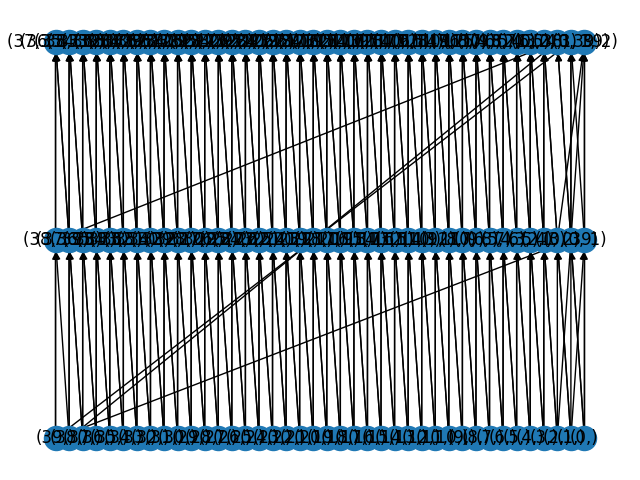
\includegraphics[width=.8\linewidth]{40.png}
      \caption{$n = 40$}
    \end{subfigure}%
    \begin{subfigure}{.5\textwidth}
      \centering
      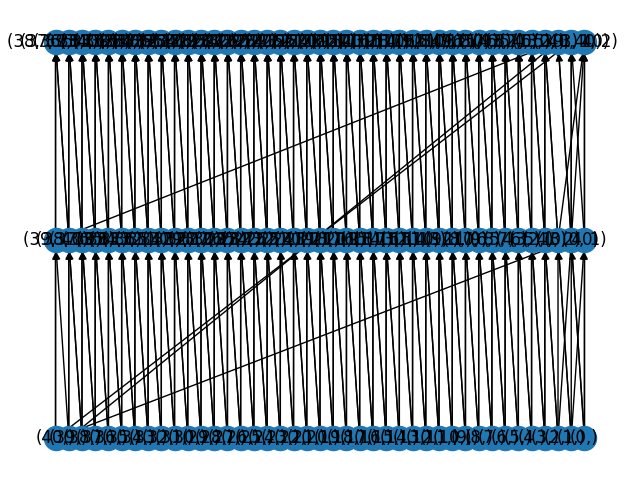
\includegraphics[width=.8\linewidth]{41.png}
      \caption{$ n = 41 $}
    \end{subfigure}
    \begin{subfigure}{.5\textwidth}
        \centering
        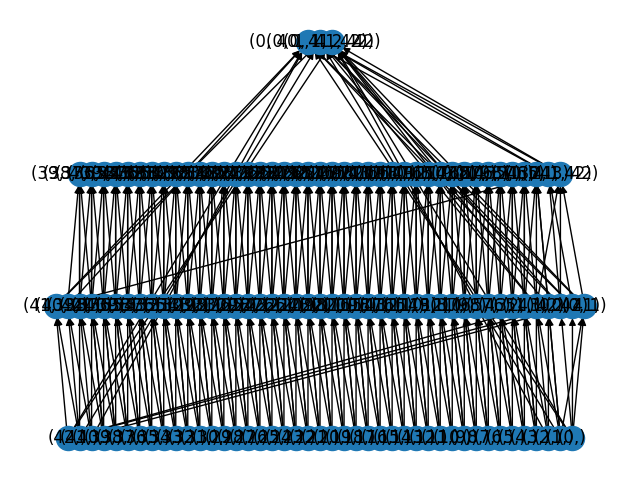
\includegraphics[width=.8\linewidth]{42.png}
        \caption{$ n = 42 $}
      \end{subfigure}%
      \begin{subfigure}{.5\textwidth}
        \centering
        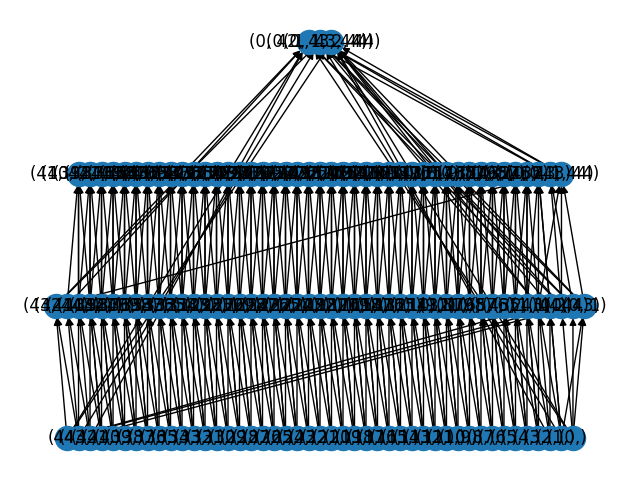
\includegraphics[width=.8\linewidth]{44.png}
        \caption{$ n = 44 $}
      \end{subfigure}
\end{figure}
